This chapter gives an overview of the High-Luminosity LHC upgrade of the LHC in Section \ref{section:hl-lhc}, and the upgrades for the Phase-2 CMS Level-1 (L1) Trigger in Section \ref{section:phase-2-l1t}. One of the major upgrades is the new availability of calorimeter crystal-level information to the L1 calorimeter trigger, compared to the current trigger which only has access to tower-level information (a tower being 5 by 5 in crystals). To capitalize on the increased spatial granularity of this information, an upgraded algorithm is presented which reconstructs and identifies electron and photon candidates in the the Layer-1 Calorimeter Trigger. A description of the algorithm and a validation of its performance in Phase-2 conditions is given in Section \ref{section:standalone_barrel_calo_egamma}.

\section{The High-Luminosity LHC}
\label{section:hl-lhc}
In order to sustain and extend the LHC's physics discovery program and maintain operability for a decade or more, the LHC is undergoing a major upgrade to the High-Luminosity LHC (HL-LHC). In its final configuration, the HL-LHC will deliver a peak luminosity of $7.5 \times 10^{34}$ cm$^{-2}$ s$^{-1}$, potentially leading to total integrated luminosity of 4000 fb$^{-1}$ after ten years of operations, scheduled to begin in 2027~\cite{CMS-TDR-021}. This integrated luminosity is about ten times the predicted luminosity reach of the LHC in its initial configuration. To enable the CMS experiment to continue operations and data-taking and to maximize the discovery potential of the unprecedented amount of data, the CMS detector is undergoing Phase-2 upgrades in order to perform high-precision measurements and searches for physics beyond the Standard Model in the intense running conditions of the HL-LHC. 

\section{The Phase-2 Level-1 Trigger}
\label{section:phase-2-l1t}
To achieve the goals of the HL-LHC program and to ensure the collection of information-rich datasets in the HL-LHC, the Phase-2 upgrade of the CMS Level-1 Trigger~\cite{CMS-TDR-021} must be upgraded in conjunction with the CMS sub-detectors and their readouts, to maintain physics selectivity. The HL-LHC will produce an intense hadronic environment corresponding to 200 simultaneous collisions per beam crossing, necessitating comprehensive upgrades of the trigger system outlined below.

In order to cope with the increased pile-up and high occupancies of the HL-LHC, the latency of the L1 trigger system (time available to produce a L1 Accept signal) will be increased significantly from 3.8 $\mu$s to 12.5 $\mu$s, with an increased maximum output bandwidth of 750 kHz~\cite{CMS-TDR-021}. With the increased latency, in addition to information from calorimeters and muon detectors (as in the Phase-1 system), information from the new tracker and high-granularity endcap calorimeter can also be included at L1 for the first time. This is illustrated in the functional diagram of the architecture of the Phase-2 trigger system in Fig. \ref{fig:phase-2-l1-architecture}. 

\begin{figure}[ht]
    \centering
    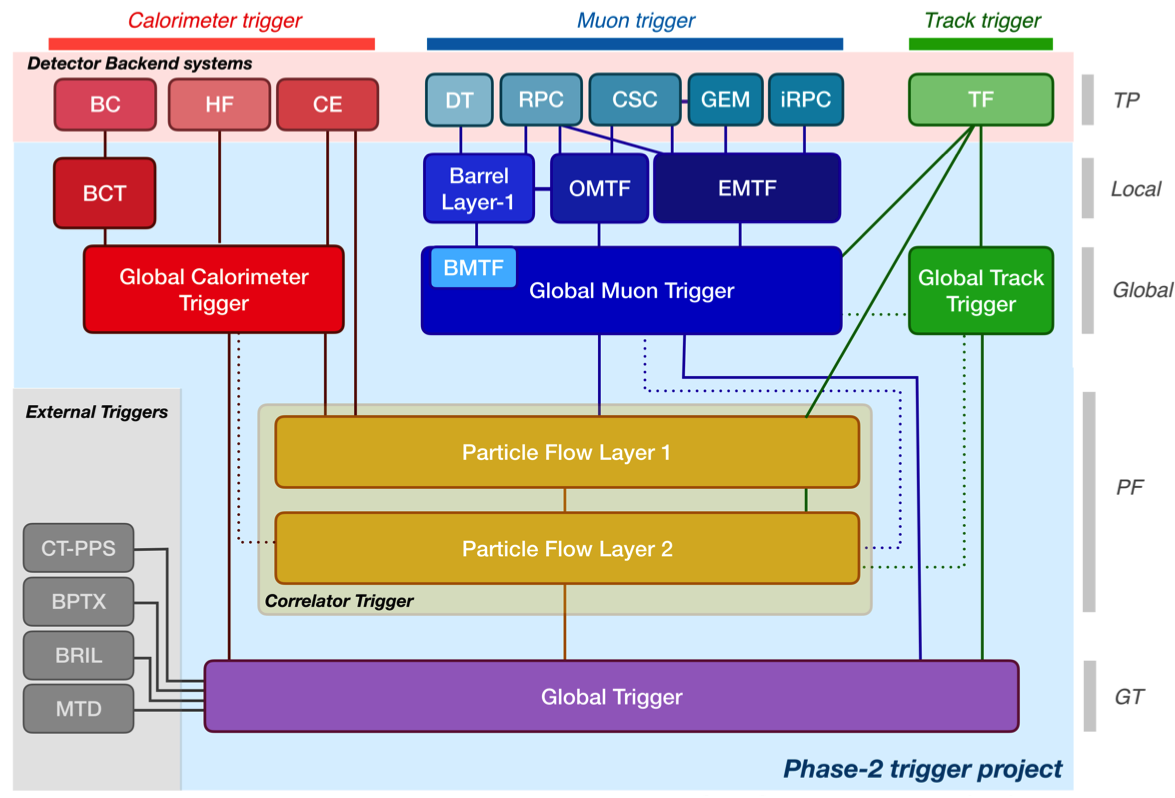
\includegraphics[width=15cm]{figures/ch-3-phase2/phase-2-l1-architecture.png}
    \caption[Functional diagram of the CMS L1 Phase-2 upgraded trigger design.]{Functional diagram of the CMS L1 Phase-2 upgraded trigger design~\cite{CMS-TDR-021}, showing the four trigger paths: calorimeter, muon, track, and Particle Flow. For the first time, tracking information will be available as early as the L1 Trigger.}
    \label{fig:phase-2-l1-architecture}
\end{figure}

The key feature of the Phase-2 L1 Trigger is the introduction of a correlator layer, where algorithms produce higher-level trigger objects by combining information from sub-detectors, with a selectivity approaching that of offline reconstruction in the HLT~\cite{CMS-TDR-021}. Four independent data processing paths (grouped together in Fig. \ref{fig:phase-2-l1-architecture}) are implemented: tracking, calorimetry, muon systems, and particle-flow techniques:
\begin{itemize}
    \item \textbf{Calorimeter Trigger path:} (\textit{red}, Fig. \ref{fig:phase-2-l1-architecture}) A barrel calorimeter trigger (BCT) and the HGCAL backend are used to process crystal-level information from the calorimeters to produce high-resolution clusters and identification variables used for later processing. Outputs from the BCT, HGCAL, and the HF are sent to a global calorimeter trigger (GCT), where calorimeter-only objects such as $e/\gamma$ candidates, hadronically decaying tau lepton candidates, jets, and energy sums are built.
    \item \textbf{Track Trigger path:} (\textit{green}, Fig. \ref{fig:phase-2-l1-architecture}) Tracks from the Outer Tracker are reconstructed in the track finder (TF) processors as part of the detector backend. A global track trigger (GTT) will reconstruct the primary vertices of the event, along with tracker-only based objects, such as jets and missing transverse momentum.
    \item \textbf{Muon Trigger path:} (\textit{blue}, Fig. \ref{fig:phase-2-l1-architecture}) Trigger primitives are processed by muon track finder algorithms, again separated into the barrel (barrel muon track finder, BMTF), overlap (overlap muon track finder, OMTF), and endcap (endcap muon track finder, EMTF). Standalone muons and stubs containing information such as position, bend angle, and timing, as well as L1 tracks, are sent to the global muon trigger (GMT).
    \item \textbf{Particle-Flow Trigger path:} (\textit{yellow}, Fig. \ref{fig:phase-2-l1-architecture}) The correlator trigger (CT) aims to approach the performance of offline Particle Flow, and is implemented in two layers. ``Layer-1'' produces the particle-flow candidates from matching calorimeter clusters and tracks. ``Layer 2'' builds and sorts final trigger objects and applies additional identification and isolation criteria.
\end{itemize}

The outputs from the above trigger paths are combined in the Global Trigger (GT) (\textit{purple}, Fig. \ref{fig:phase-2-l1-architecture}), which calculates the final trigger decision (Level-1 Accept), transmitting it to the Trigger Control and Distribution System (TCDS), which distributes it to the detector backend systems, initiating the readout to the DAQ. The GT also provides the interface to external triggers (\textit{grey}, Fig. \ref{fig:phase-2-l1-architecture}), such as triggers for the precision proton spectrometer (PPS), beam position and timing monitors (BPTX), and luminosity and beam monitoring (BRIL) detectors~\cite{CMS-TDR-021}. The design of the Phase-2 Level-1 Trigger allows for future inclusion of triggering information, for instance information about minimum ionizing particles (MIPs) from the MIP Timing Detector (MTD)~\cite{CERN-LHCC-2017-027}.

\section{Standalone Barrel Calorimeter electron/photon reconstruction}
\label{section:standalone_barrel_calo_egamma}
The reconstruction and identification of electrons and photons ($e/\gamma$) begin with the trigger primitives of the barrel ECAL and HCAL detectors and endcap HGCAL calorimeters, covering the pseudorapidity region $|\eta| < 3$. The barrel and endcap regions of the detector are intrinsically different enough to warrant different approaches to $e/\gamma$ reconstruction. This work presents a firmware-based emulator for the standalone $e/\gamma$ reconstruction in the barrel calorimeter (Fig. \ref{fig:phase-2-summary-trigger-TP-algo-physics}). ``Standalone" refers to the fact that the tracker information is not used in this particular reconstruction chain. This firmware-based emulator is based on the parallelized, computational logic that will be deployed in the firmware of the Phase-2 Level-1 trigger. The emulator uses fixed-precision integers to represent all values, such as in the computation of cluster energies, and closely mimics the firmware logic which uses arrays and performs computations in flattened loops. It represents an improved, more realistic understanding of the trigger, compared to the previous emulator which used idealized logic such as vector operations, and floats to represent all values~\cite{CMS-TDR-021}.

\begin{figure}[ht]
    \centering
    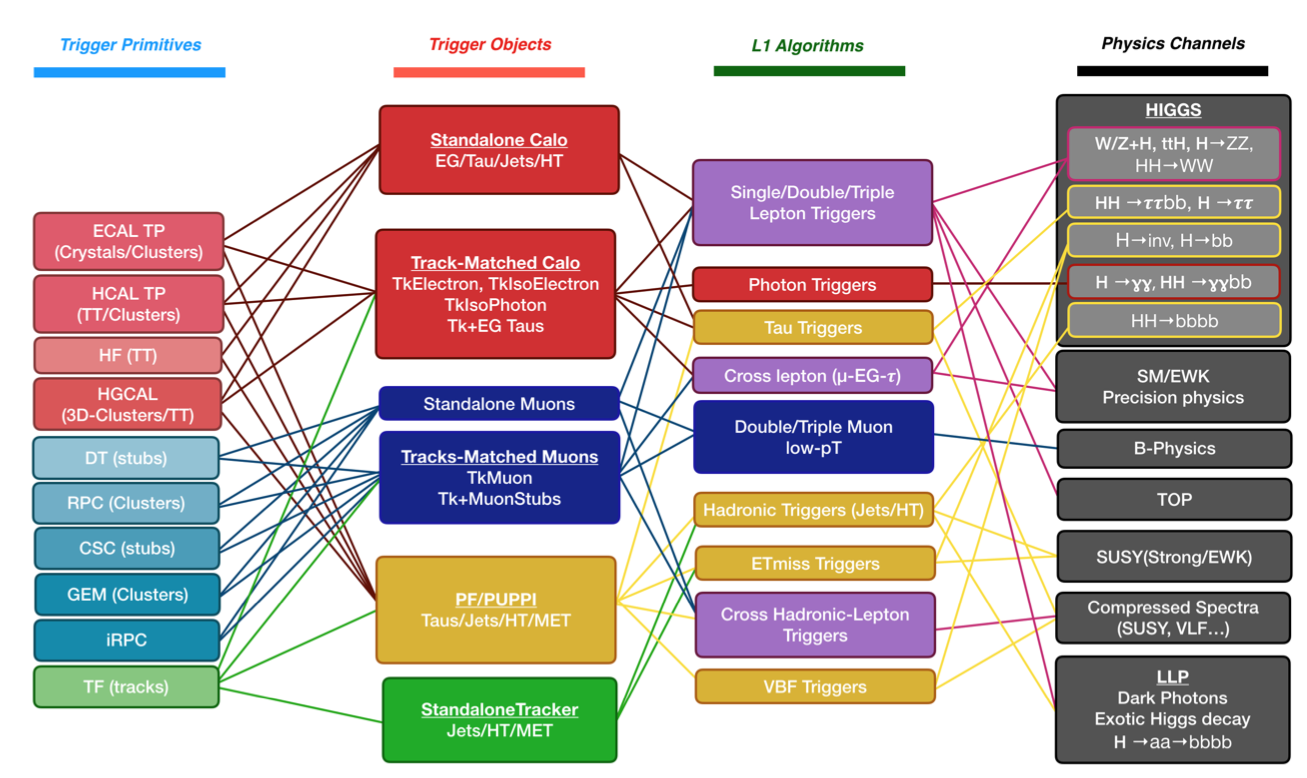
\includegraphics[width=15cm]{figures/ch-3-phase2/phase-2-summary-trigger-TP-algo-physics.png}
    \caption[Summary of the links between the trigger primitives, the trigger objects, the Level-1 algorithms, and the physics channels in the Phase-2 menu.]{Summary of the links between the trigger primitives (\textit{first column}), the trigger objects (\textit{second column}), the Level-1 algorithms used in the menu (\textit{3rd column}), and the physics channels (\textit{4th column}), from~\cite{CMS-TDR-021}, where a full description of the Phase-2 L1 algorithms can be found. This work focuses on developments for the Standalone Calorimeter electron and photon ("EG") reconstruction algorithm.}
    \label{fig:phase-2-summary-trigger-TP-algo-physics}
\end{figure}

\subsection{Electron/photon standalone barrel procedure}
% https://cds.cern.ch/record/2714892/files/CMS-TDR-021.pdf  
% Section 2.2.1, on page 36-37
In Phase-2, the upgrade of both on-detector and off-detector electronics of the barrel calorimeters' trigger primitive generator (TPG) will enable the streaming of single crystal data from the on-detector to the backend electronics. Currently in Phase-1, the ECAL and HCAL TPGs is restricted to providing lower-granularity information of trigger tower sums of $5 \times 5$ crystals to the Level-1 Trigger~\cite{CMS-TDR-021}. A schematic of the geometry of the ECAL barrel in the Phase-2 Regional Calorimeter Trigger (RCT) is shown in Fig. \ref{fig:phase-2-rct-cards-schematic}. The barrel is spanned by 36 RCT cards, each spanning $17 \times 4$ towers in $\eta \times \phi$. Each RCT card is subdivided into five ``regions'' as shown in Fig. \ref{fig:phase-2-one-rct-card-schematic-landscape}.  After initial clustering and processing, the outputs of the RCT card are sent to the Global Calorimeter (GCT) trigger, which is processed in three cards as shown in Fig. \ref{fig:phase-2-gct-cards-schematic}. The reconstruction algorithm is detailed below.
\begin{figure}[!ht]
    \centering
    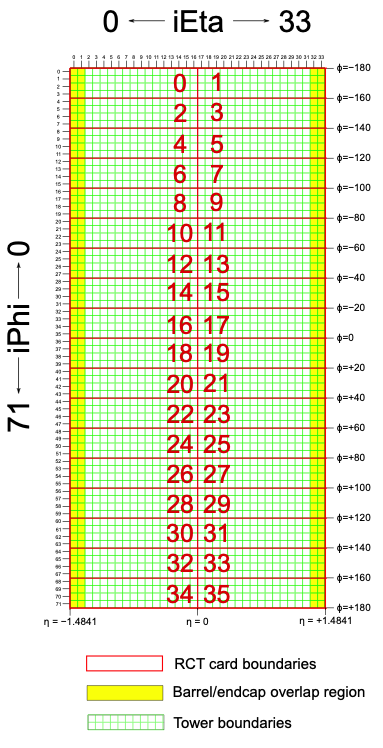
\includegraphics[width=5cm]{figures/ch-3-phase2/phase-2-rct-cards-schematic.png}
    \caption{Schematic of the geometry of the Phase-2 ECAL barrel in the Regional Calorimeter Trigger (RCT), showing the division of the barrel region into 36 Regional Calorimeter Trigger (RCT) cards (\textit{red}). Each card spans $17 \times 4$ towers in $\eta \times \phi$ (\textit{green}), and each tower is $5\times 5$ in single crystals in $\eta \times \phi$. Towers in the overlap region (\textit{shaded yellow}) are read out to both the barrel and endcap.}
    \label{fig:phase-2-rct-cards-schematic}
\end{figure}


\begin{figure}[ht]
    \centering
    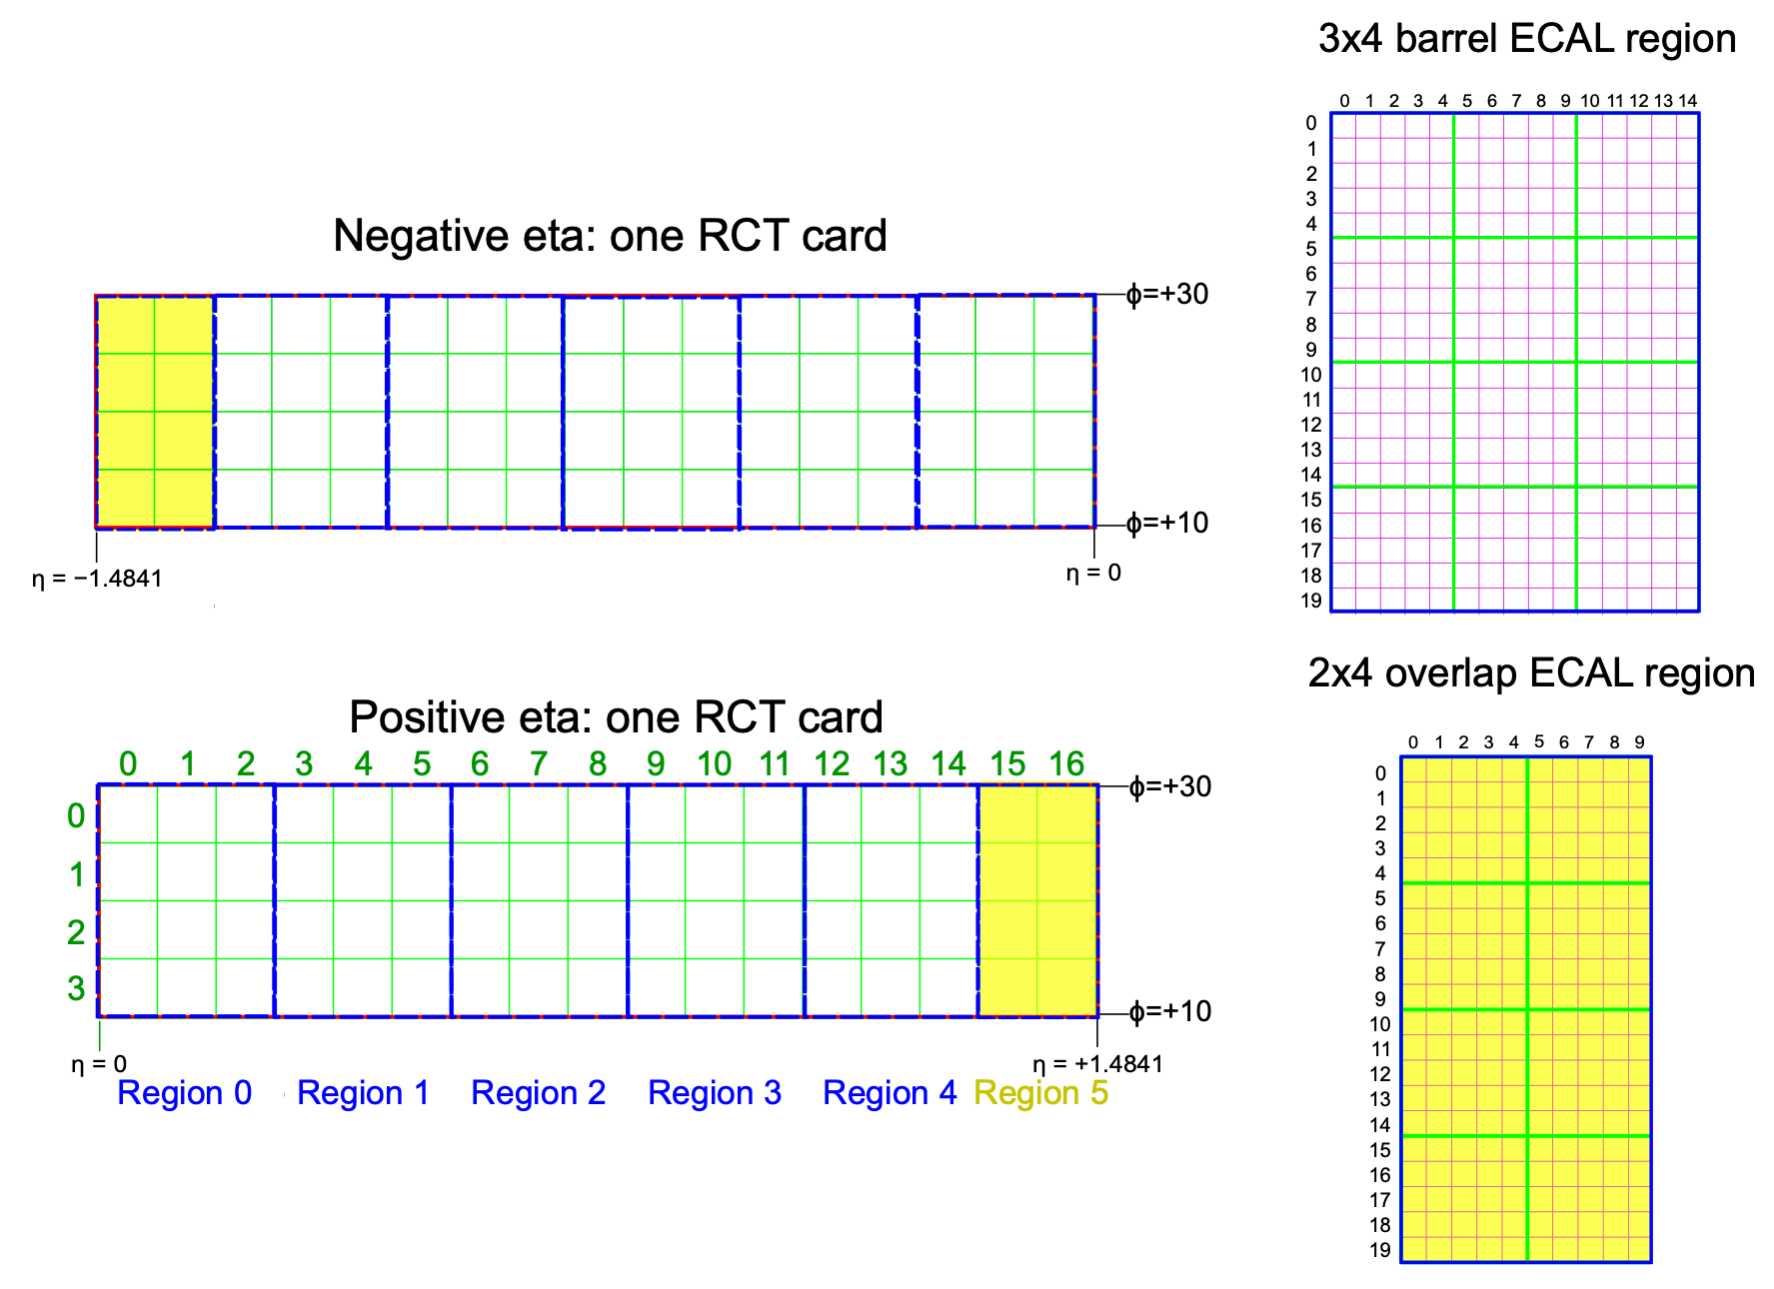
\includegraphics[width=11cm]{figures/ch-3-phase2/phase-2-one-rct-card-schematic-landscape.png}
    \caption{Schematic of two example RCT cards in the negative eta (\textit{top left}) and positive eta (\textit{bottom left}) regions of the ECAL barrel. Each RCT card is divided into six regions: five regions are of size $3 \times 4$ towers in $\eta \times \phi$ (\textit{top right}), and a sixth smaller overlap region of size $2 \times 4$ towers (\textit{bottom right}). Each tower is $5 \times 5$ ($\eta\times\phi$) in crystals.}
    \label{fig:phase-2-one-rct-card-schematic-landscape}
\end{figure}


\begin{figure}[ht]
    \centering
    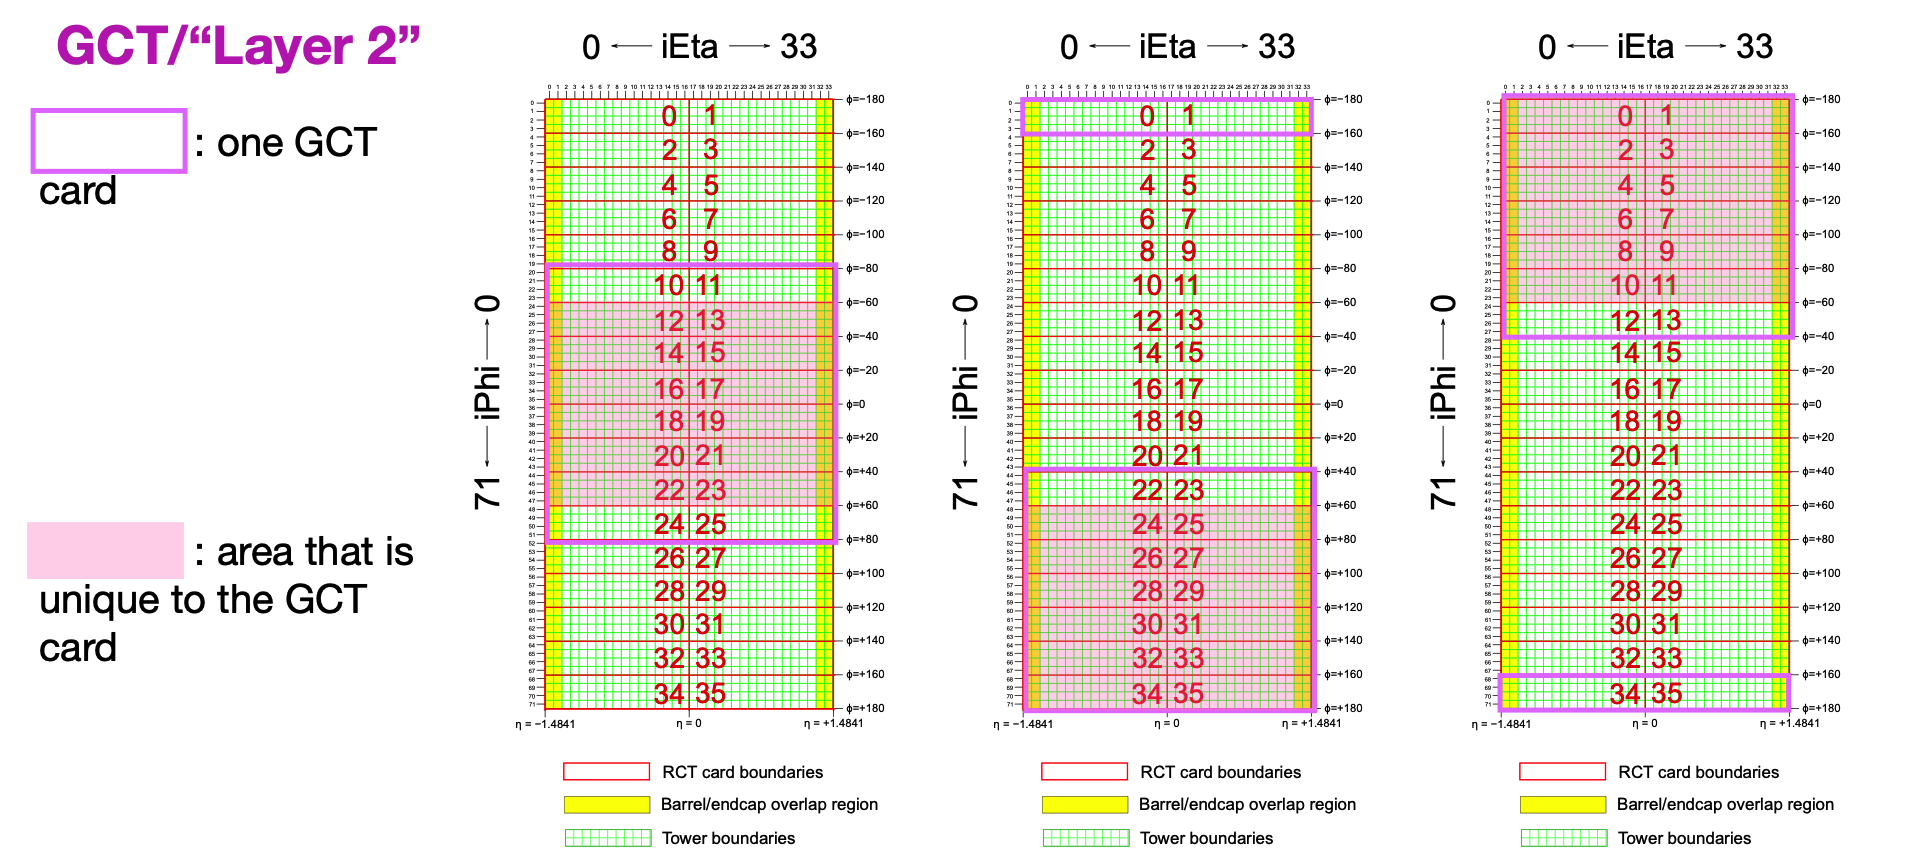
\includegraphics[width=15cm]{figures/ch-3-phase2/phase-2-gct-cards-schematic.png}
    \caption{Schematic of the Phase-2 ECAL barrel in the Global Calorimeter Trigger (GCT), which will process the outputs of the Regional Calorimeter Trigger (RCT) in three GCT cards (\textit{purple borders}). Each card in the GCT processes the equivalent of sixteen RCT cards, with the center twelve RCT cards being unique to that GCT card (\textit{shaded pink}), and the remaining four RCT cards overlapping with one other GCT card.}
    \label{fig:phase-2-gct-cards-schematic}
\end{figure}

The standalone barrel algorithm for reconstructing and identifying electrons and photons in the Phase-2 Level-1 Trigger takes as input the digitized response of each crystal of the barrel ECAL, with a granularity $0.0175 \times 0.0175$ in $\eta \times \phi$, which is 25 times higher than the input to the Phase-1 trigger, which consisted of trigger towers with a granularity of $0.0875 \times 0.0875$. In HCAL the tower size of $0.0875 \times 0.0875$ is unchanged. The trigger algorithm is designed to closely reproduce the algorithm used in the offline reconstruction, with limitations and simplifications due to trigger latency. 

\begin{figure}[ht]
    \centering
    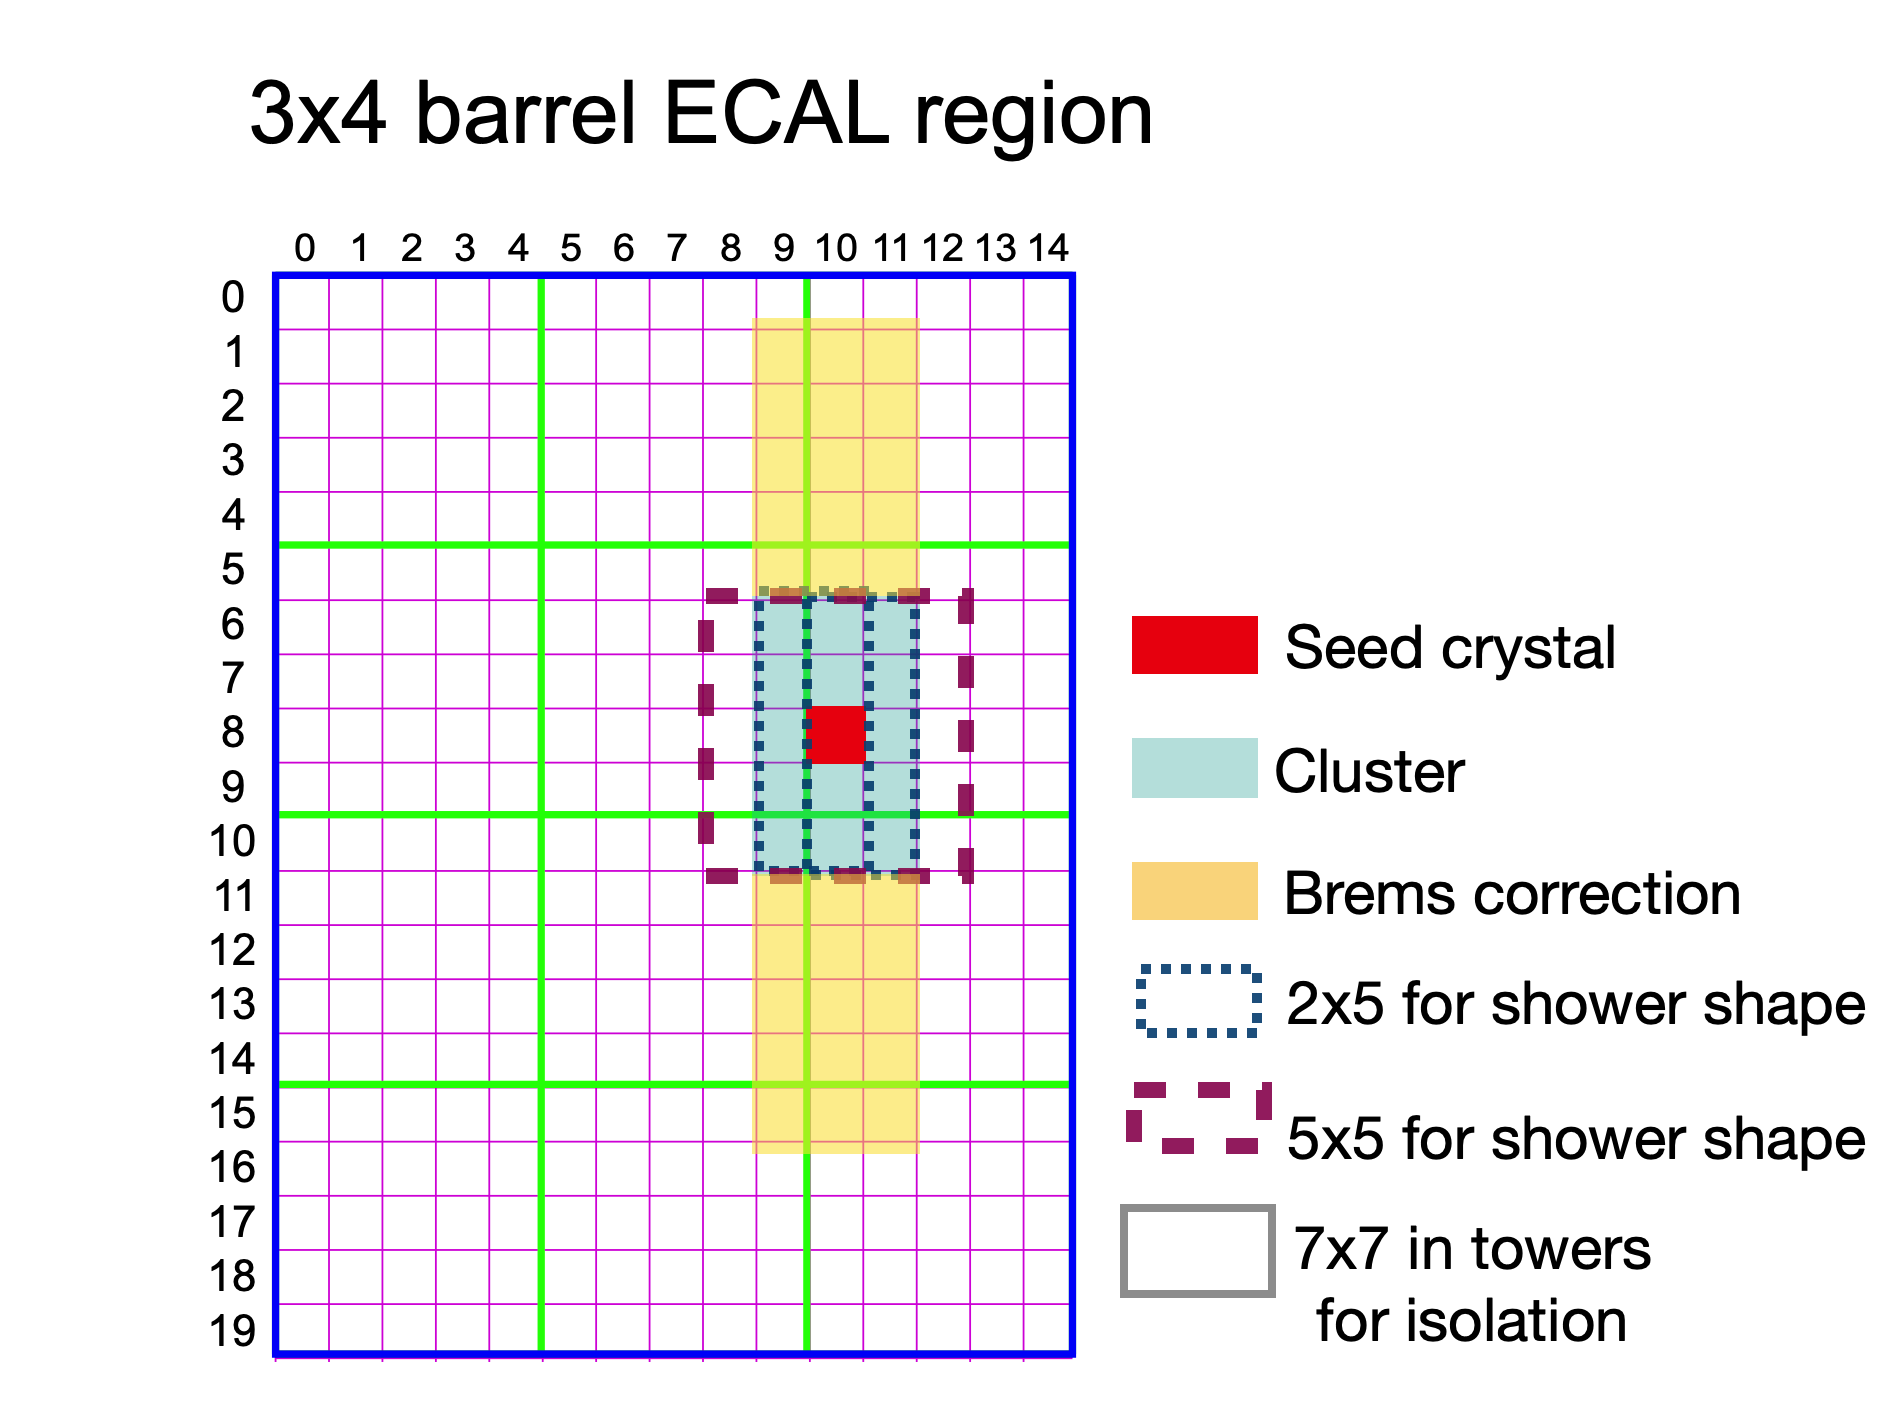
\includegraphics[width=12cm]{figures/ch-3-phase2/phase-2-cluster-footprint.png}
    \caption{Illustration of an example electron/photon ($e/\gamma$) cluster in the Phase-2 Level-1 Trigger standalone barrel $e/\gamma$ reconstruction, in a region of $15\times 20$ crystals ($3\times 4$ towers) in $\eta \times \phi$. Each small pink square is one crystal, the highest-granularity ECAL trigger primitives available to the L1 Trigger in Phase-2. The core cluster consists of the energy sum in a $3\times 5$ window of crystals (\textit{shaded light blue}), centered around the seed crystal (\textit{red}). The presence of energy lost to bremsstrahlung radiation is checked in the adjacent $3\times 5$ windows in the $\phi$ direction (\textit{shaded light yellow}). The ratio of the total energies in windows of size $2\times 5$ and $5\times 5$ in crystals (\textit{dashed dark blue and dark red}) around the seed crystal, is computed and compared to the core cluster energy to obtain shower shape flags. Lastly, the isolation, defined as the sum of the energy in a large window of size $7\times 7$ in towers (not shown in figure) is computed, and compared to the core cluster energy to obtain isolation flags.}
    \label{fig:phase-2-cluster-footprint}
\end{figure}


In the RCT, an initial requirement of $p_{T} > 0.5$ GeV is imposed on the input trigger primitives (i.e. energies from the ECAL crystals and HCAL towers) to reject contribution from pile-up. In one of the regions inside a RCT card (Fig. \ref{fig:phase-2-one-rct-card-schematic-landscape}), the crystal containing the highest energy deposit is identified as the seed crystal, as shown in Fig. \ref{fig:phase-2-cluster-footprint}. The energy in the crystals in a window of size $3\times 5$ in $\eta\times\phi$ around the seed cluster is added into a cluster. The energy is considered ``clustered''. The process is repeated with the remaining ``unclustered" energy, until up to four clusters are produced in the region. 

To improve $e/\gamma$ identification and to reduce background contributions, identification and reconstruction algorithms are implemented at this stage:
\begin{itemize}
    \item Shower shape: The energy deposit sums around the seed crystal is computed in windows of size $2 \times 5$ and $5 \times 5$ (Fig. \ref{fig:phase-2-cluster-footprint}, \textit{dashed lines}), with true $e/\gamma$ clusters tending to produce showers that deposit most of their energy in a $2 \times 5$ region. 
    \item Bremsstrahlung recovery: $e/\gamma$ tend to spread in the $\phi$ direction due to charged particles being bent by the magnetic field of the CMS solenoid. If sufficient energy comparable to the core $3 \times 5$ cluster is found in the adjacent $3 \times 5$ windows (Fig. \ref{fig:phase-2-cluster-footprint}, \textit{shaded yellow}), the energy is added to the core cluster and no longer considered unclustered energy.
\end{itemize}

After parallel processing in the regions, the clusters in a RCT card are stitched together if they are located directly along the borders of a region (Fig. \ref{fig:phase-2-rct-cards-schematic}). The remaining unclustered ECAL energy is summed into ECAL towers. 

From each RCT card, the twelve highest-energy clusters, as well as any remaining unclustered energy, are sent to the GCT. Since each GCT card has information from sixteen RCT cards (Fig. \ref{fig:phase-2-gct-cards-schematic}), final stitching across the boundaries of the RCT cards is performed. One more identification algorithm is performed at this stage:
\begin{itemize}
    \item Isolation: One handle to reject backgrounds from e.g. pile-up, comes from the tendency for background to be spread more uniformly across a large area in the detector, whereas genuine $e/\gamma$ are expected to produce showers concentrated in the $3 \times 5$ crystal window. The energy sum in a large window of $7 \times 7$ in towers is computed and used to reject background.
\end{itemize}
Flags that provide discrimination power between genuine $e/\gamma$ and background, are computed using the relative isolation and shower shape quantities. The standalone working point (WP) is defined as the logical OR of the relative isolation and shower shape flags. 

\subsection{Electron/photon standalone barrel output and results}
The performance of the current emulator of the standalone barrel $e/\gamma$ algorithm in Phase-2 conditions is quantified in efficiencies and rates. Efficiency is the fraction of true electrons that the algorithm can reconstruct and identify, and is evaluated in a Monte Carlo simulated sample containing electrons with transverse momentum $p_{T}$ ranging from 1 to 100\GeV.  The efficiencies of the current and previous emulaors as a function of the electron generator-level $p_{T}$ are shown in Fig. \ref{fig:results-egamma-efficiency-gt25}. 

The rates are the event rates that this reconstruction and identification algorithm would obtain if it were deployed in a trigger, assuming that proton-proton collisions are occurring at the 40 MHz event rate of the HL-LHC. The rate is reported as a function of the minimum energy threshold required by the trigger, and is estimated using a simulated sample of minimum bias events, i.e. generic proton-proton collisions without any specific physics selections. The rates for the current and previous emulator are shown in Fig. \ref{fig:results-egamma-rates}. 

\begin{figure}[ht]
    \centering
    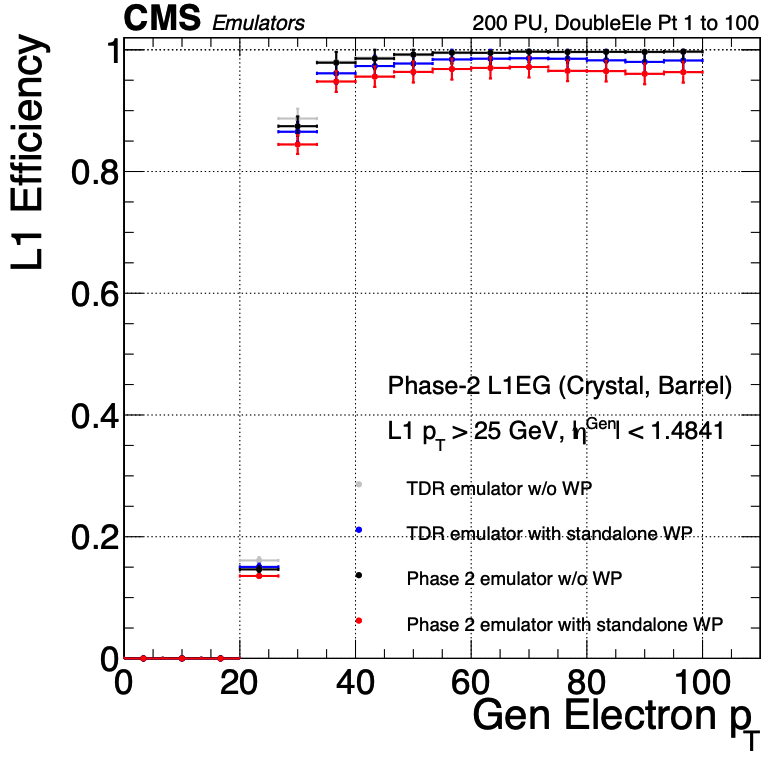
\includegraphics[width=12cm]{figures/ch-3-phase2/results-egamma-efficiency-gt25.png}
    \caption{Efficiencies of the current and previous emulators of the standalone barrel $e/\gamma$ algorithm for the Phase-2 Level-1 Trigger, evaluated in a simulated sample containing electrons, as a function of the electron's generator-level transverse momentum $p_{T}$. The standalone working point (WP) is defined as the logical OR of the isolation flag and shower shape flag. The efficiencies with and without requiring the standalone WP, are shown for the current emulator (labeled ``Phase 2", \textit{black, red}) and the previous emulator (labeled ``TDR", \textit{dark blue, grey}).}
    \label{fig:results-egamma-efficiency-gt25}
\end{figure}

\begin{figure}[h]
    \centering
    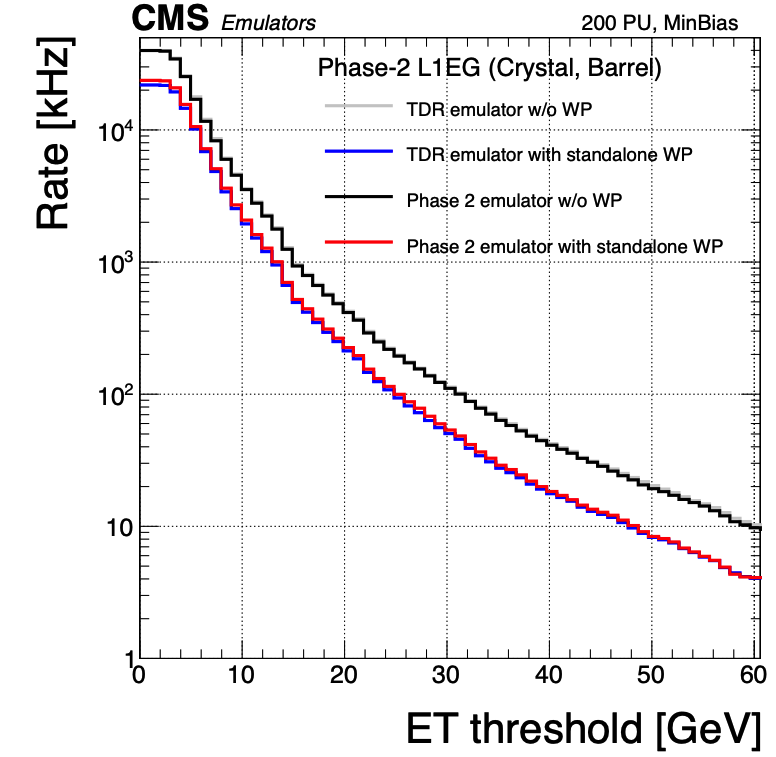
\includegraphics[width=12cm]{figures/ch-3-phase2/results-egamma-rates.png}
    \caption{Rates in kHz of the current Phase-2 and previous (``TDR") emulators of the standalone barrel $e/\gamma$ algorithm for the Phase-2 Level-1 Trigger, evaluated on a minimum bias (MinBias) sample with 200 pile-up (PU), measured as a function of the minimum energy ($E_T$) required of the reconstructed $e/\gamma$ object in each event. The standalone working point (standalone WP) is defined to be the logical OR of the isolation flag and the shower shape flag. The rates with and without requiring the standalone WP, are shown for the current emulator (labeled ``Phase 2", \textit{black, red}) and the previous emulator (labeled ``TDR", \textit{dark blue, grey}).}
    \label{fig:results-egamma-rates}
\end{figure}

% TODO: discuss performance in menu

The information of the clusters in the event, including their energies, crystal-level position, the relative isolation flag, the shower shape flag, the standalone WP, and the ratio of the HCAL over ECAL energies, are sent in digitized ``words" of 64 bits to the Correlator Trigger and the Global Trigger. The towers in the event are computed as the sum of all unclustered energy in the ECAL with the corresponding HCAL energy at each tower location, and their energies are sent to the Correlator Trigger.

% TODO: talk about how the outputs are used